\chapter{Moving Solitons in the Lugiato-Lefever equation.}

In section~\ref{sec:fra_LS} we introduced the concept of dissipative localized structures (LSs). Here, we will study the formation
of such structures in nonlinear optical systems where they are often called optical or cavity solitons. 
More specifically, we will analyze the paradigmatic Lugiato-Lefever equation (LLE) \cite{lugiatolefever1987} used to describe fiber resonators, and
study the formation of LSs when a fourth order derivative and a non-local term are considered.


\section{Lugiato-Lefever equation.}

In 1987, Lugiato and Lefever proposed a simple yet extremely rich nonlinear partial differential equation to study the formation of patterns and localized states
in the framework of nonlinear optics \cite{lugiatolefever1987}. They considered a cavity filled with a nonlinear medium in the low transmission (or high quality) limit
driven by a continuous wave. In order to keep the equation as simple as possible, they considered a cubic nonlinearity which is characteristic of Kerr media. Moreover,
In virtue of the low dissipation limit, they originally neglected the longitudinal variable $z$ (along which light propagates) and kept only the transversal plane $x-y$ as spatial
variables in the equation. In contrast, a longitudinal (or temporal) LLE was later formulated by Haelterman and his colleagues [ref], where only the longitudinal 
coordinate becomes relevant. The main difference between these two equations is that in the former, a transversal Laplacian appears due to diffraction of the light, whereas
in the latter, a longitudinal Laplacian appears due to dispersion of the light. However, from a mathematical point of view, they are the same equations.


\begin{equation}
    \dfrac{\partial E}{\partial t} = E_{in} - (1 + i\theta) E + i |E|^2 E + i\nabla^2 E
    \label{lle:lle}
\end{equation}

In our case, we will consider the longitudinal LLE corresponding to Eq.~(\ref{lle:lle}) as a starting point and we will analyze
the effect of adding a fourth order dispersion term and the Raman effect which will be explained in the following section.

\section{Raman effect.}

Raman effect frequently observed 26-31. 

Stabilization of LSs by means of the Raman effect. 39, 41, 41-43 in normal dispersion and far from MI. 

\section{Isolas and traveling solitons.}

In that case the LS is formed due to front locking between the two CW solutions (i.e. it requires bistability). 
However, in this case the LS arise due to coexistence between periodic state and CW, so even in the monostable can be observed.

\begin{SCfigure}
    \centering
    \caption{asdasd}
    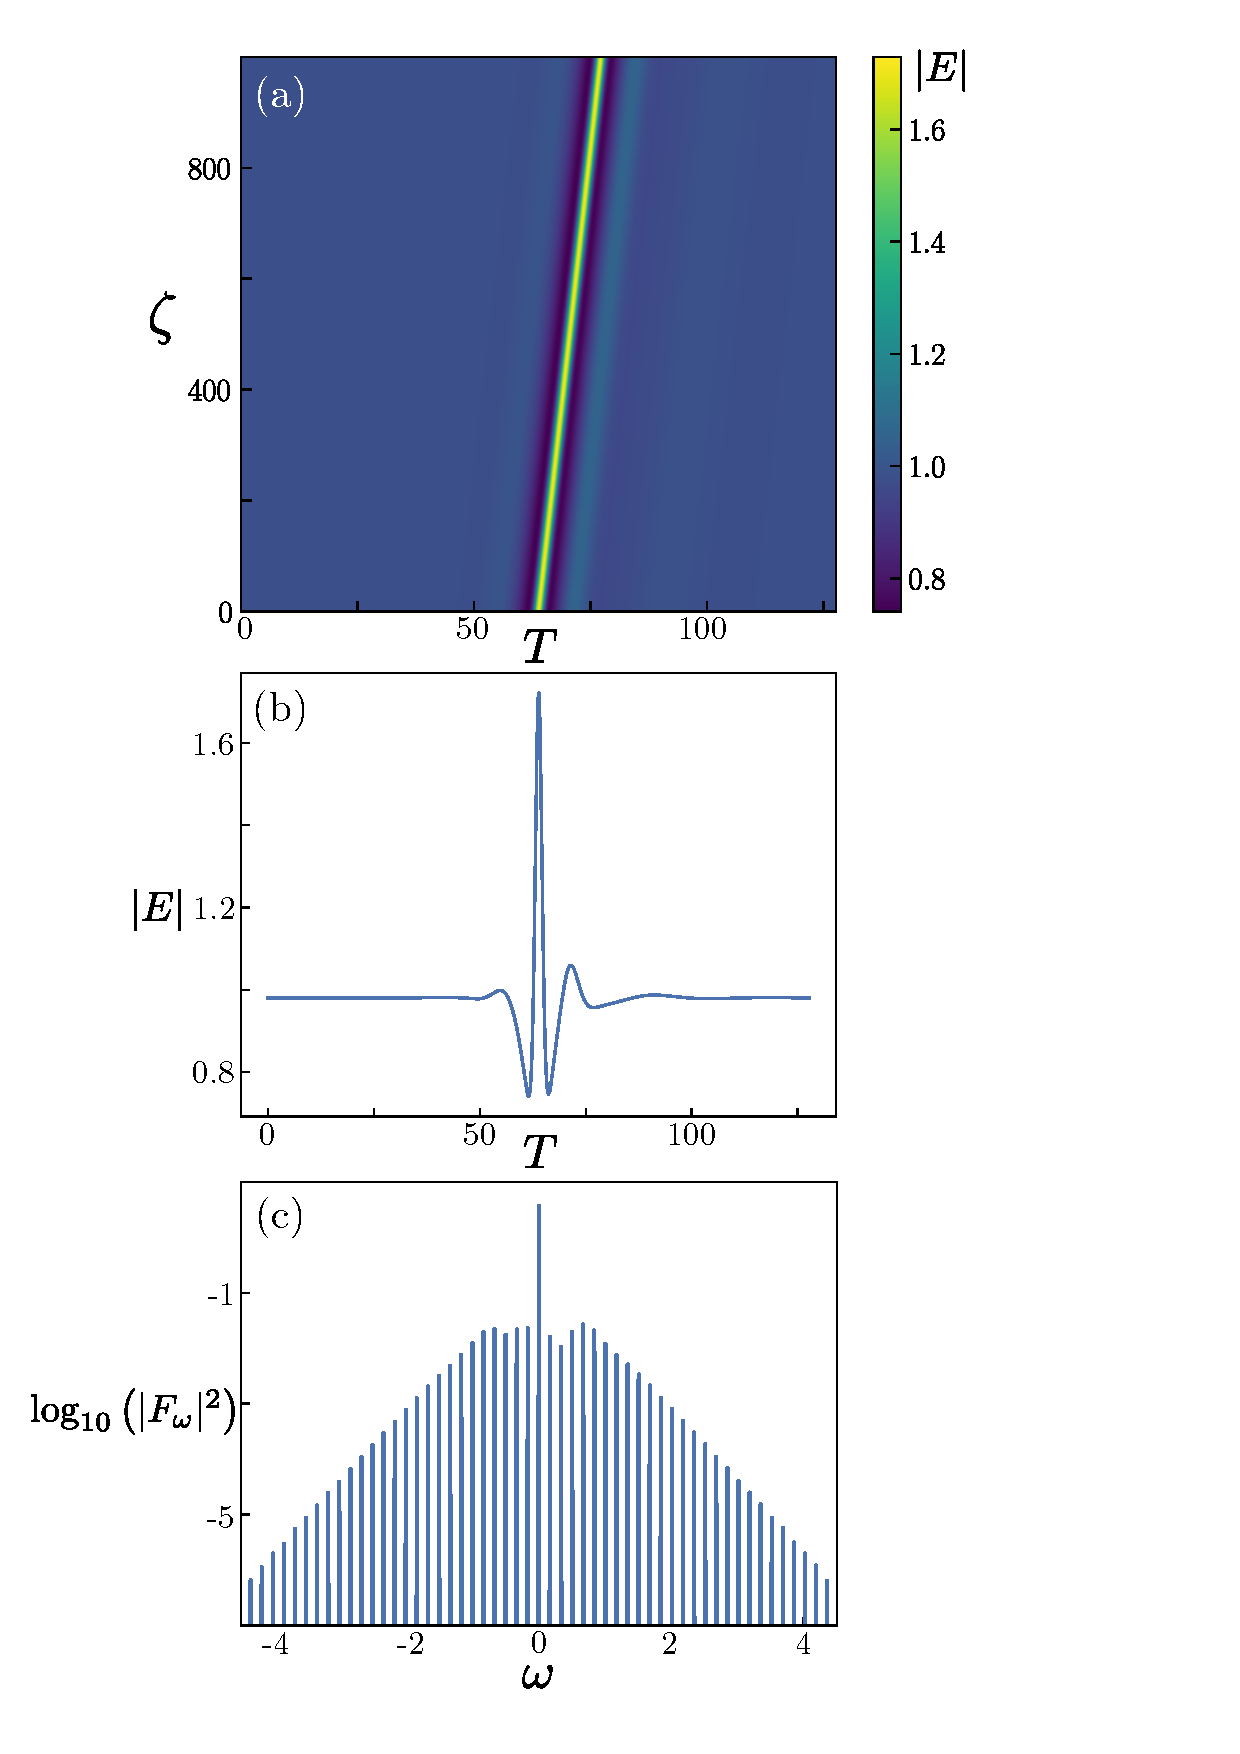
\includegraphics[width=0.6\textwidth]{imagenes/lle/LLE_Spatiotemporal.pdf}
\end{SCfigure}

\begin{figure}
    \centering
    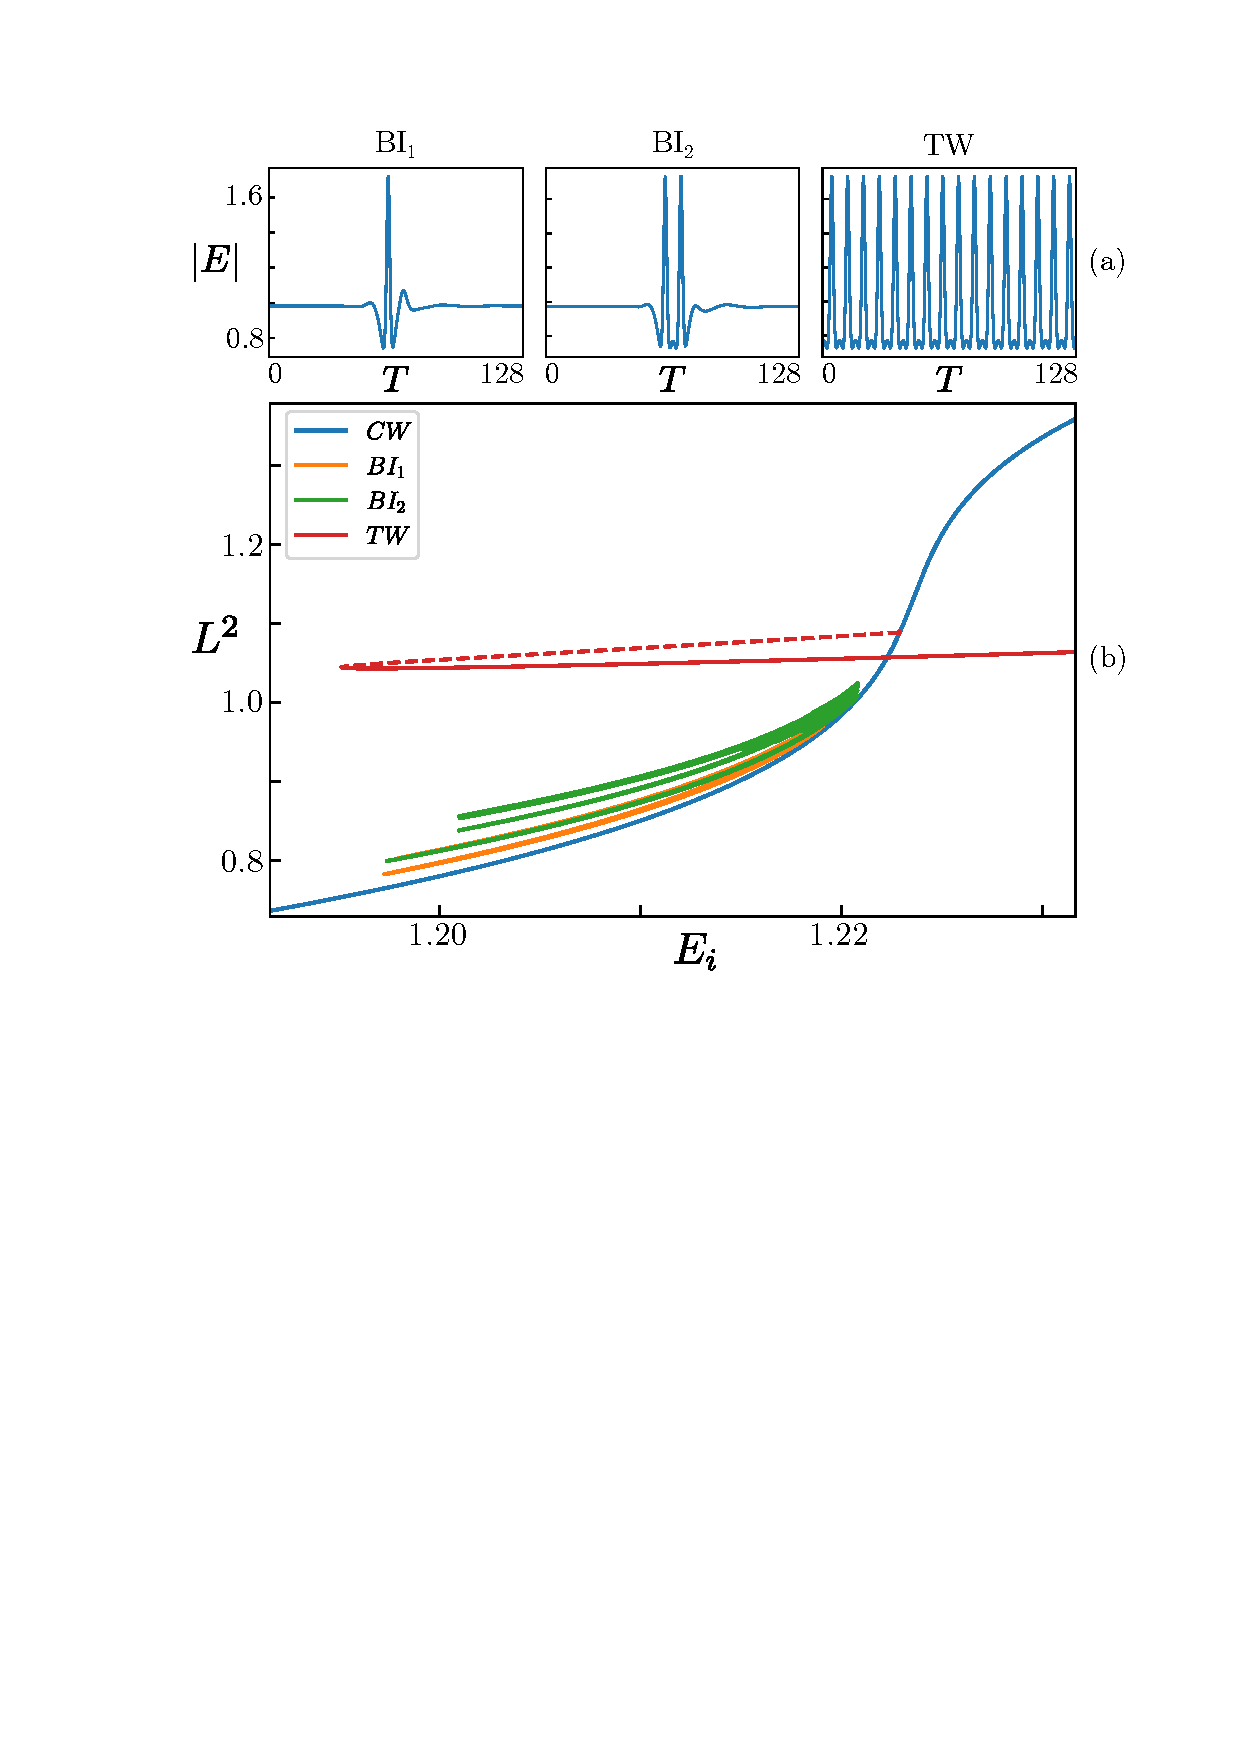
\includegraphics[width=0.7\textwidth]{imagenes/lle/LLE_Isola.pdf}
    \caption{asd}
\end{figure}

\section{A reduced model.}

\begin{SCfigure}
    \centering
    \caption{asdasd}
    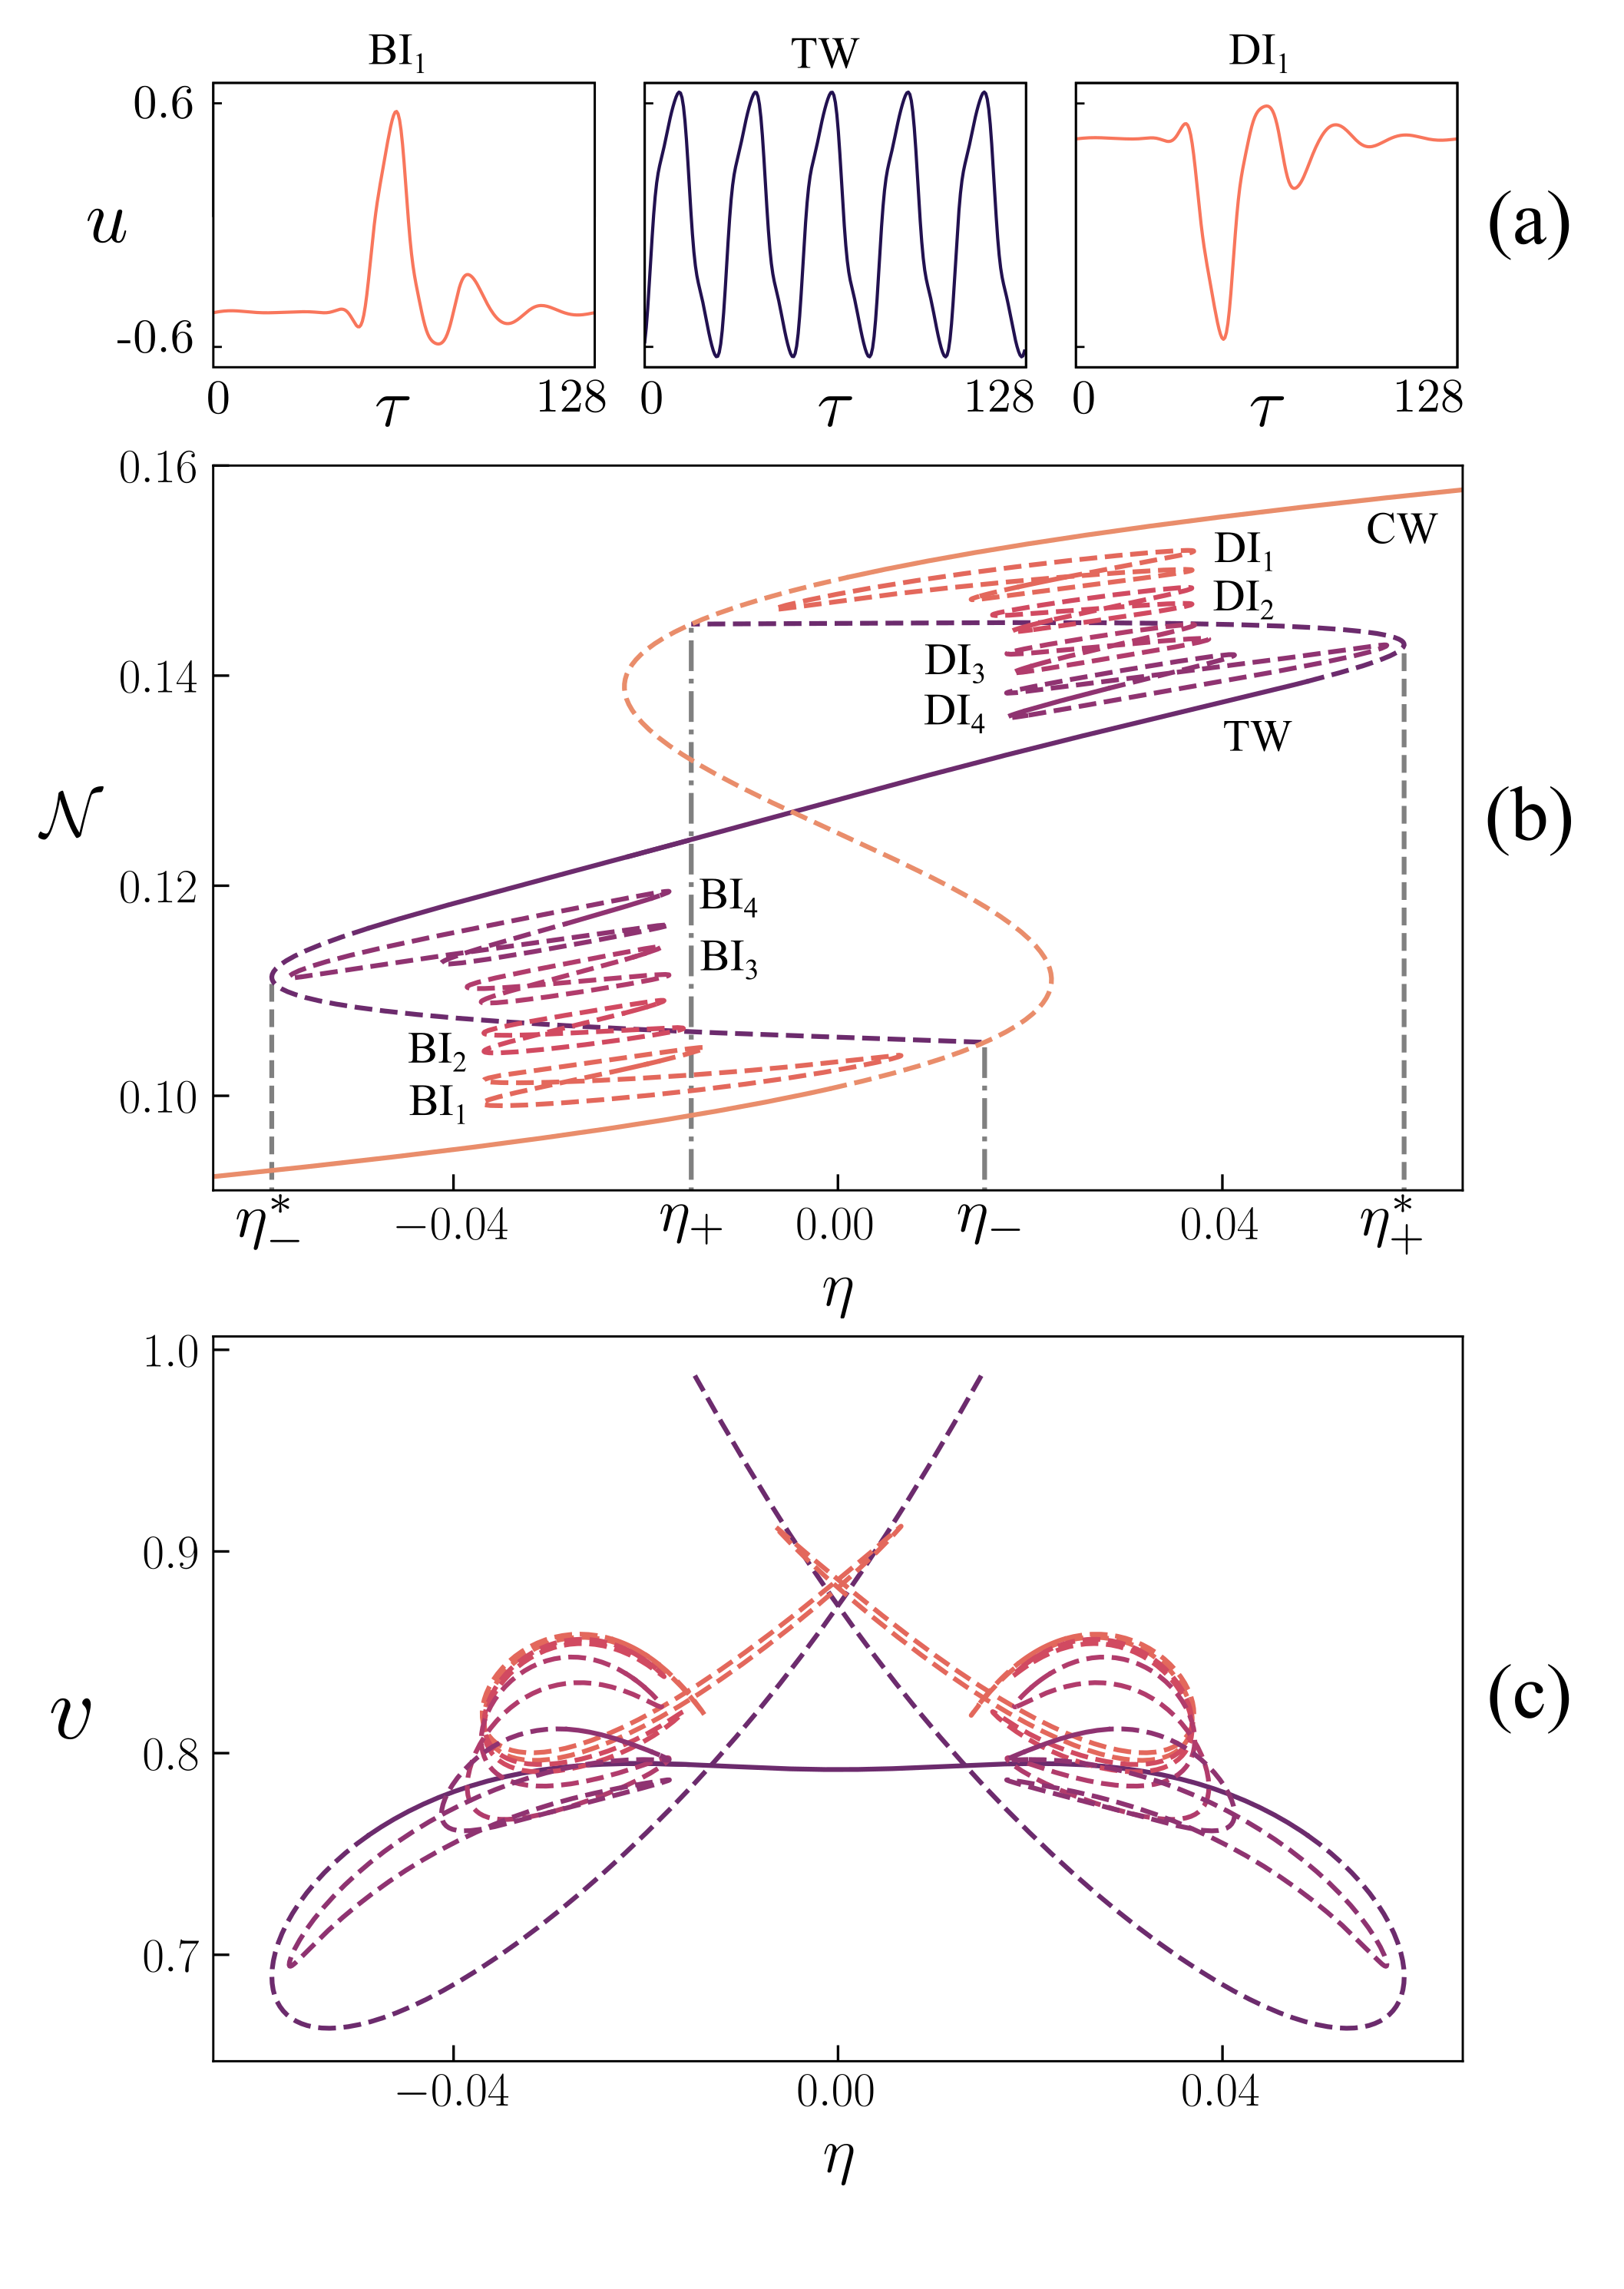
\includegraphics[width=0.6\textwidth]{imagenes/lle/Fig3.png}
\end{SCfigure}

\begin{figure}[h]
    \centering
    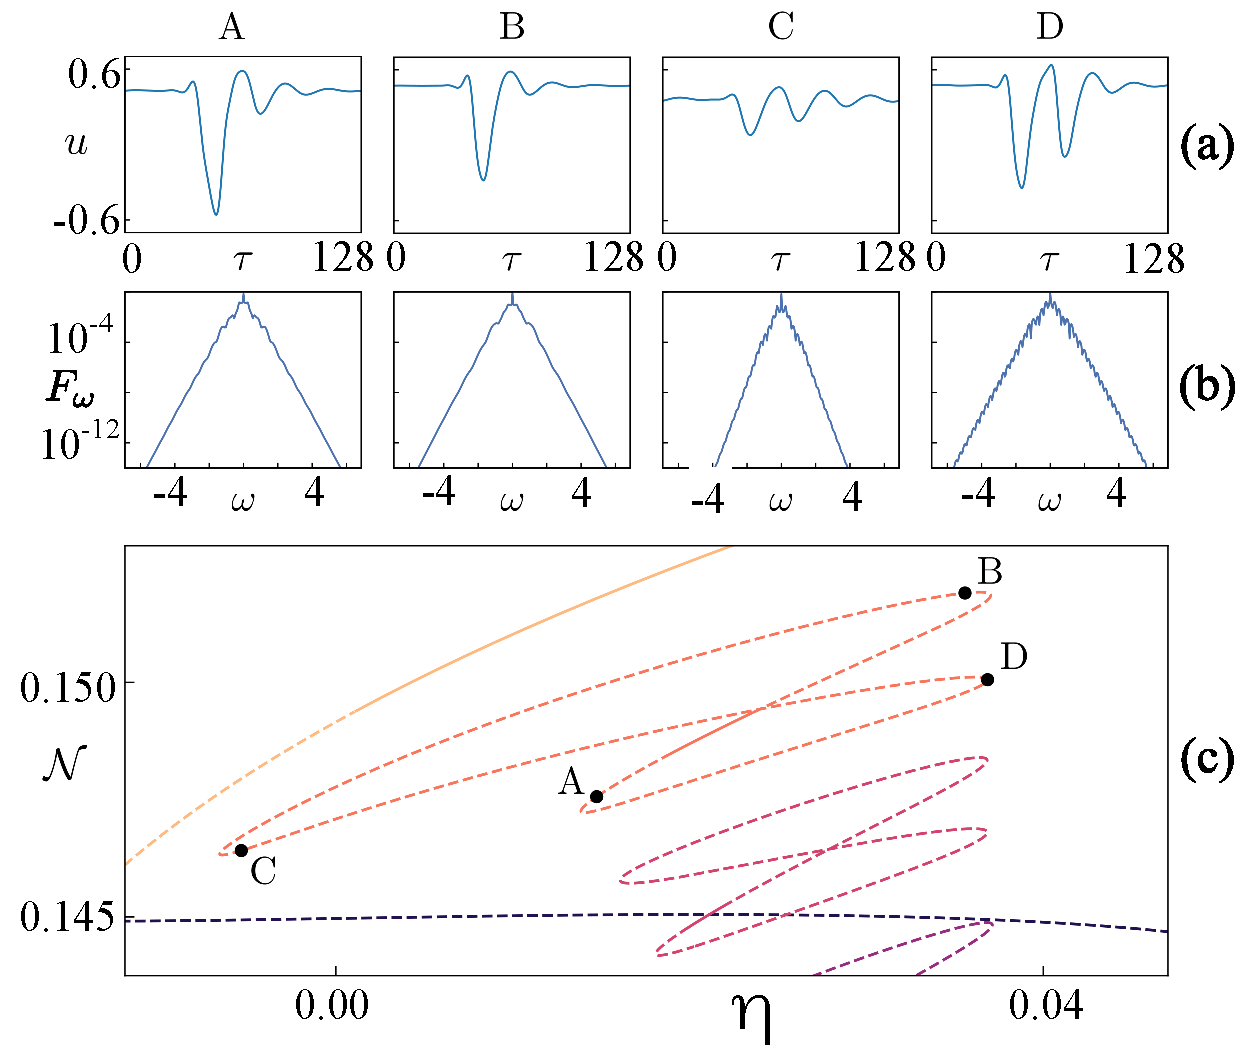
\includegraphics[width=0.5\textwidth]{imagenes/lle/Fig4-Isola.pdf}
    \caption{asd}
\end{figure}

\section{Oscillatory bound states.}

\begin{enumerate}
    \item 
\end{enumerate}